

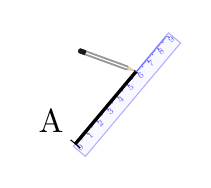
\begin{tikzpicture}[scale=0.2,rotate=50,every node/.style={scale=1.2}]

%début de la règle
    %Graduaton max. de la règle
    \def \Taille {9}
    %Définition de l 'angle de rotation de la règle
    \def \Rotation {0}
    %Définition du décalage de la règle
    \def \DecalX {0}
    \def \DecalY {0}
    %Couleur des élèments de la règle (sauf le remplissage)
    \def \RegleColor {blue!60}

\begin{scope}[scale=1,shift={(\DecalX,\DecalY)},rotate=\Rotation]
    % contours de la règle
    \draw[color=\RegleColor, fill =blue!5, opacity=0.5] (-0.2,0.5) rectangle (\Taille+0.2,-0.5);	%Dont couleur de remplissage
    % graduation 1 mm
    \foreach \a in {0,0.1,...,\Taille}{\draw[color=\RegleColor] (\a,0.5)--(\a,0.42);}
    % graduation 5 mm
    \foreach \a in {0,0.5,...,\Taille}{\draw[color=\RegleColor] (\a,0.42)--(\a,0.35);}
    % graduation et repères 10 mm
    \foreach \a in {0,1,...,\Taille}{\draw[color=\RegleColor] (\a,0.35)--(\a,0.25)
    node[scale=0.5,font=\tiny, rotate=40] (\a) at (\a,0.1){\a};}
%fin de la règle

\draw (0,0.5) node[above left]{A};
\draw (0,0.5)--+(90:0.4)--+(-90:0.4);
\draw [very thick](0,0.5)--(6,0.5);

\end{scope}

\begin{scope}[scale=0.8,xshift=7.52cm,yshift=.62cm,rotate=20] %le crayon, xshift et yshift pour les coordonnées de la pointe, rotate pour l'orientation du crayon
\def \couleur {black}
\coordinate (O) at (0,0);
\fill[\couleur!40] (-0.2,4.8) -- (0.2,4.8) -- (0.2,0.8) --(0.1,0.65) -- (0,0.8) -- (-0.1,0.66) -- (-0.2,0.8) -- cycle; %corps du crayon
\draw[color=white] (0,4.8) -- (0,0.8); %trait intérieur du crayon
\fill[\couleur!90] (-0.2,4.3) -- (0,4.27) -- (0.2,4.3) -- (0.2,4.8) arc(30:150:0.23cm); %partie haute du crayon
\fill[brown!40] (-0.2,0.8) -- (O)node[coordinate,pos=0.75](a){} -- (0.2,0.8)node[coordinate,pos=0.25](b){} -- (0.1,0.65) -- (0,0.8) -- (-0.1,0.66) -- cycle; %pointe du crayon (partie taillée)
\fill[\couleur!90] (a) -- (O) -- (b) -- cycle; %mine du crayon
\end{scope}


\end{tikzpicture}


